
%(BEGIN_QUESTION)
% Copyright 2014, Tony R. Kuphaldt, released under the Creative Commons Attribution License (v 1.0)
% This means you may do almost anything with this work of mine, so long as you give me proper credit

Calculate the output voltages of these two voltage divider circuits ($V_A$ and $V_B$):

$$\includegraphics[width=15.5cm]{i01238x01.eps}$$

Now, calculate the voltage between points {\bf A} (red lead) and {\bf B} (black lead) ($V_{AB}$).

\underbar{file i01238}
%(END_QUESTION)





%(BEGIN_ANSWER)

$V_A =$ + 65.28 V

\vskip 10pt

$V_B =$ + 23.26 V

\vskip 10pt

$V_{AB} =$ + 42.02 V (point {\bf A} being positive relative to point {\bf B})

%(END_ANSWER)





%(BEGIN_NOTES)


%INDEX% Electronics review: series and parallel circuits

%(END_NOTES)


